%%%%%%%%%%%%%%%%%%%%%%%%%%%%%%%%%%%%%%%%%
% Beamer Presentation
% LaTeX Template
% Version 1.0 (10/11/12)
%
% This template has been downloaded from:
% http://www.LaTeXTemplates.com
%
% License:
% CC BY-NC-SA 3.0 (http://creativecommons.org/licenses/by-nc-sa/3.0/)
%
%%%%%%%%%%%%%%%%%%%%%%%%%%%%%%%%%%%%%%%%%

%----------------------------------------------------------------------------------------
%	PACKAGES AND THEMES
%----------------------------------------------------------------------------------------

\documentclass{beamer}

\mode<presentation> {

% The Beamer class comes with a number of default slide themes
% which change the colors and layouts of slides. Below this is a list
% of all the themes, uncomment each in turn to see what they look like.

%\usetheme{default}
%\usetheme{AnnArbor}
%\usetheme{Antibes}
%\usetheme{Bergen}
%\usetheme{Berkeley}
%\usetheme{Berlin}
%\usetheme{Boadilla}
%\usetheme{CambridgeUS}
%\usetheme{Copenhagen}
%\usetheme{Darmstadt}
%\usetheme{Dresden}
%\usetheme{Frankfurt}
%\usetheme{Goettingen}
%\usetheme{Hannover}
%\usetheme{Ilmenau}
%\usetheme{JuanLesPins}
%\usetheme{Luebeck}
\usetheme{Madrid}
%\usetheme{Malmoe}
%\usetheme{Marburg}
%\usetheme{Montpellier}
%\usetheme{PaloAlto}
%\usetheme{Pittsburgh}
%\usetheme{Rochester}
%\usetheme{Singapore}
%\usetheme{Szeged}
%\usetheme{Warsaw}

% As well as themes, the Beamer class has a number of color themes
% for any slide theme. Uncomment each of these in turn to see how it
% changes the colors of your current slide theme.

%\usecolortheme{albatross}
%\usecolortheme{beaver}
%\usecolortheme{beetle}
%\usecolortheme{crane}
%\usecolortheme{dolphin}
%\usecolortheme{dove}
%\usecolortheme{fly}
%\usecolortheme{lily}
%\usecolortheme{orchid}
%\usecolortheme{rose}
%\usecolortheme{seagull}
%\usecolortheme{seahorse}
%\usecolortheme{whale}
%\usecolortheme{wolverine}

%\setbeamertemplate{footline} % To remove the footer line in all slides uncomment this line
%\setbeamertemplate{footline}[page number] % To replace the footer line in all slides with a simple slide count uncomment this line

%\setbeamertemplate{navigation symbols}{} % To remove the navigation symbols from the bottom of all slides uncomment this line
}

\usepackage{graphicx} % Allows including images
\usepackage{booktabs} % Allows the use of \toprule, \midrule and \bottomrule in tables

%----------------------------------------------------------------------------------------
%	TITLE PAGE
%----------------------------------------------------------------------------------------

\title[Newton Bases and PDEs]{Kernel Newton Bases for solving PDEs} % The short title appears at the bottom of every slide, the full title is only on the title page

\author{Tim McCollam, Palmer Lao} % Your name
\institute[IIT, CU] % Your institution as it will appear on the bottom of every slide, may be shorthand to save space
{
Illinois Institute of Technology, Clarkson University \\ % Your institution for the title page
\medskip
\textit{tmccolla@hawk.iit.edu, laopa@clarkson.edu} % Your email address
}
\date{\today} % Date, can be changed to a custom date

\begin{document}

\begin{frame}
\titlepage % Print the title page as the first slide
\end{frame}

%----------------------------------------------------------------------------------------
%	PRESENTATION SLIDES
%----------------------------------------------------------------------------------------


\begin{frame}
\frametitle{Motivation}
\begin{itemize}
\item Standard interpolation: given a set of data $f(x_i)=\{x_1, x_2, ... x_n\}$, find a function $s(x)$ that exactly fits all of these points.
\item According to a paper by Robert Schaback (2011), there exists a basis called the Newton Basis which has better conditioning than the typical Kernel Basis.
\item Palmer's stuff here
\end{itemize}
\end{frame}


\begin{frame}
\frametitle{Newton Basis}
\begin{itemize}
\item We want basis functions $v$ such that
	\begin{itemize}
	\item $v_j(x_i)=0$ for $i<j$
	\item $v_j(x_j)=1$
	\item span$\{v_1, ... v_n\}=$ span$\{k_1, ... k_n\}$ where the $k_i$'s are the standard Kernel Basis.
	\end{itemize}
\item We calculate the Newton Matrix with $\beta_{ij}=K(x_i,x_j)-\sum\limits^{i-1}_{k=0}{\beta_{jk}v_{k}(x_i)}$
\begin{itemize}
\item Where $\beta_{ij}$ is the element in the $i$th row, $j$th column of the Newton Matrix,  and $v_j(x) = \prod_{i=0}^{j-1}(x-x_i)$.
\end{itemize}
\end{itemize}
\end{frame}

\begin{frame}
\frametitle{Condition Numbers}
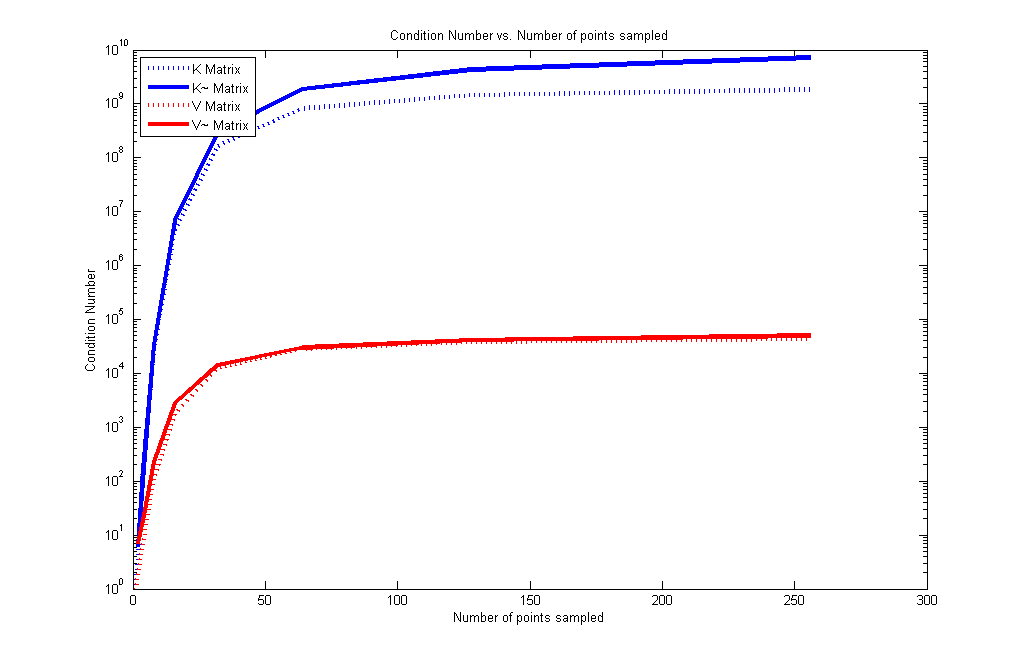
\includegraphics[scale = .45]{condNum}
\end{frame}

\begin{frame}
\frametitle{Interpolation}
\begin{itemize}
\item Interpolation with the Newton Basis is very similar to interpolation with the Kernel Basis.
\item Normally, the function is approximated by $\tilde{f}(x)=\textbf{k}^{T}\underline{K}^{-1}\textbf{y}$ (power functions).
\item Simply replace the Kernel Matrix and Vector with the Newton Matrix and Vector.
\end{itemize}
\end{frame}

\begin{frame}
\frametitle{Interpolation and Absolute Error}
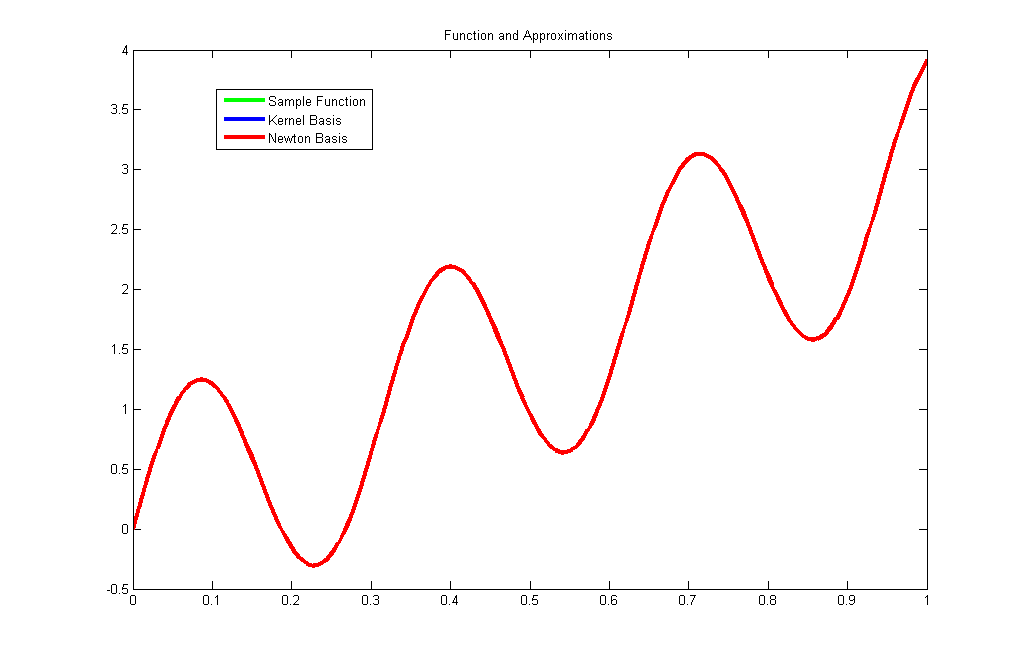
\includegraphics[scale = .45]{functionAppx}
%put interpolation graph here
\end{frame}

\begin{frame}
\frametitle{Interpolation and Absolute Error}
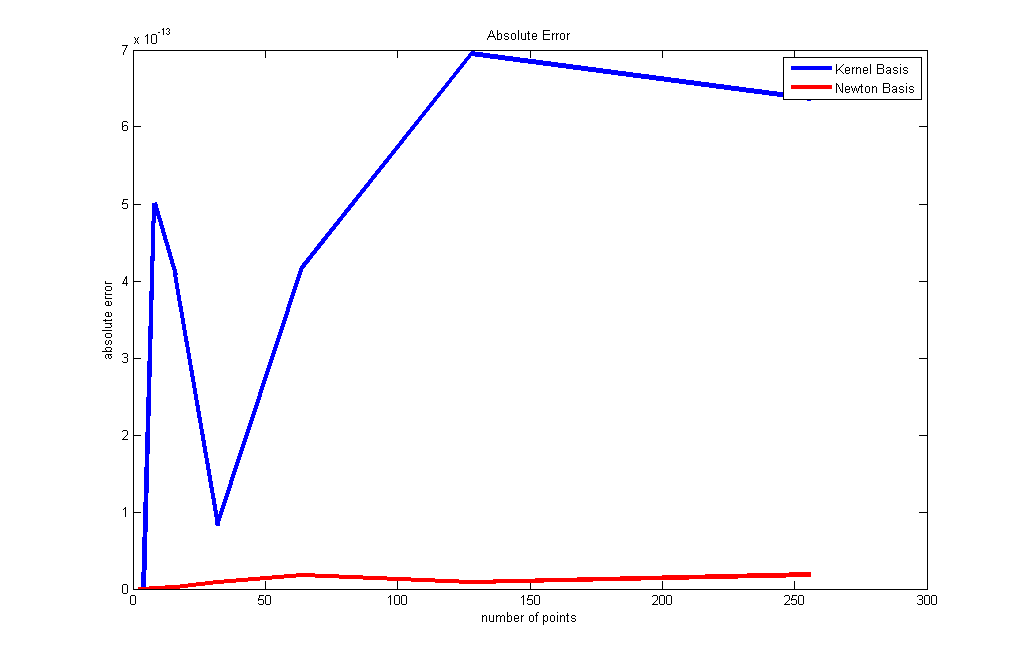
\includegraphics[scale =.45]{functionError}
%put error graph here
\end{frame}

%------------------------------------------------

\begin{frame}
\Huge{\centerline{Thanks!}}
\end{frame}

%----------------------------------------------------------------------------------------

\end{document} 